%_____________________________________________________________________________________________ 
% LATEX Template: Department of Comp/IT BTech Project Reports
% Sample Chapter
% Sun Mar 27 10:25:35 IST 2011
%
% Note: Itemization, enumeration and other things not shown. A sample figure is included.
%_____________________________________________________________________________________________ 

\chapter{Implementation}
\section{Technologies used}
\subsection{Python} 
Python is a widely used high-level, general-purpose, interpreted, dynamic programming language. Python supports multiple programming paradigms, including object oriented, imperative and functional programming or procedural styles.
Entire application is written in python including both front end and back end. 
\subsection{wxPython}
\textit{wxPython} is a GUI toolkit for the Python programming language. It allows Python programmers to create programs with a robust, highly functional graphical user interface with ease. 

\textit{wxPython} is used for all the UI components. \textit{wx.grid}, \textit{wx.StaticText}, \textit{wx.Panel}, \textit{wx.ComboBox} are some of the important classes used in front end.
\subsection{Wxwidgets}
\textit{Wxwidgets} gives you a single, easy-to-use API for writing GUI applications on multiple platforms that still utilize the native platform's controls and utilities.
\textit{WxPython} is a python wrapper over \textit{Wxwidgets}. It makes extensive use of \textit{Wxwidgets} under the hood.
\subsection{Python modules}
\begin{itemize}
\item {\bfseries Pickle :} \textit{pickle} module implements a fundamental, but powerful algorithm for serializing and de-serializing a Python object structure.
\item {\bfseries Ezodf :} \textit{ezodf} is a Python package to create new or open existing OpenDocumentFormat files to extract, add, modify or delete document data.
\item {\bfseries Pdfkit :} \textit{wkhtmltopdf} python wrapper to convert html to pdf using the webkit rendering engine
\end{itemize}


\newpage
\section{Front-end}
GUI consist of a grid i.e. a table which is used in typical timetables. Basic constraints and header information can be provided through a window. WxPython provides classes \textit{wx.grid} class for the table UI and \textit{wx.Dialog} class for windowing purposes.

\begin{figure}[ht!]
	\centering
	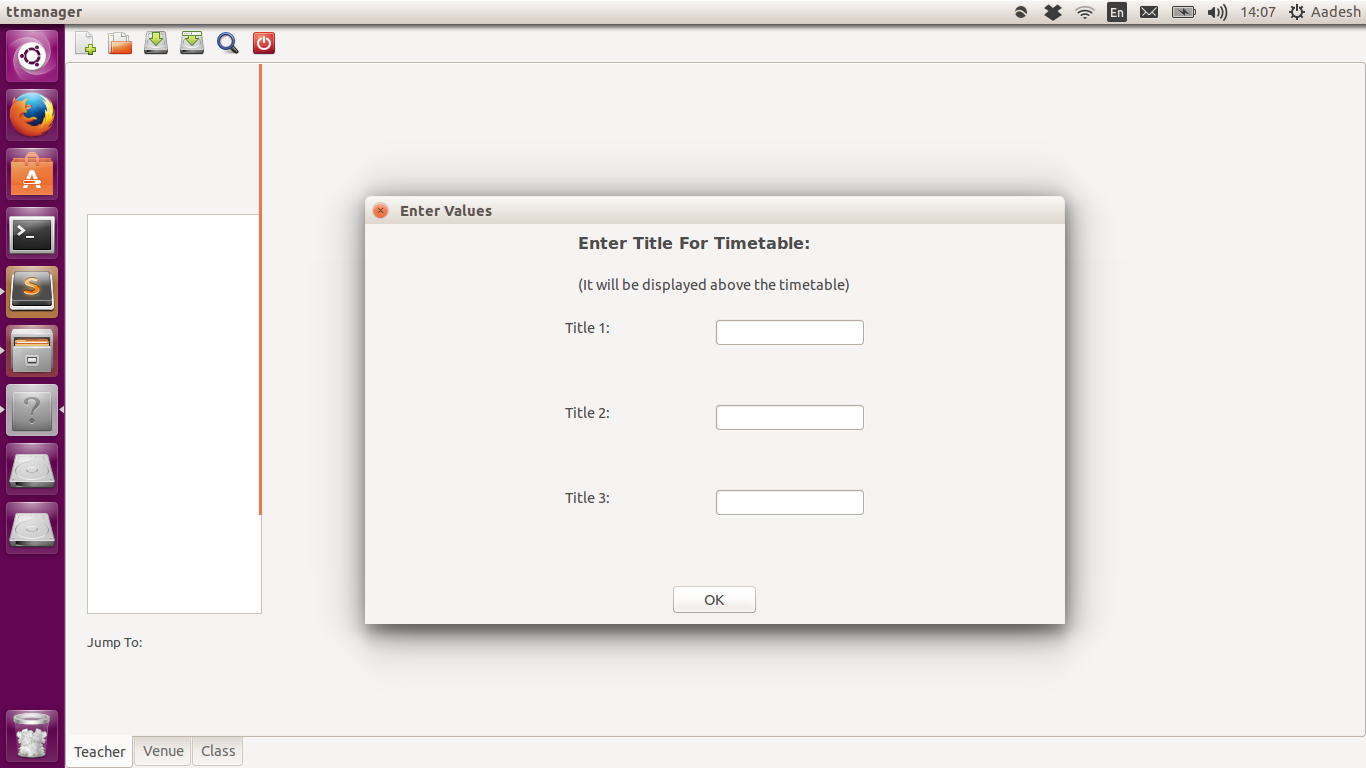
\includegraphics[width=140mm]{2.png}
	\caption{Header Information}
\end{figure}

Separate windows are available to enter teacher, venue, class and subject data. A window to enter teacher-subject, teacher-class, venue-class mappings is available. The class \textit{wx.ListCtrl} is used for all list related UI.

\newpage
An example of teacher data entry.
\begin{figure}[ht!]
	\centering
	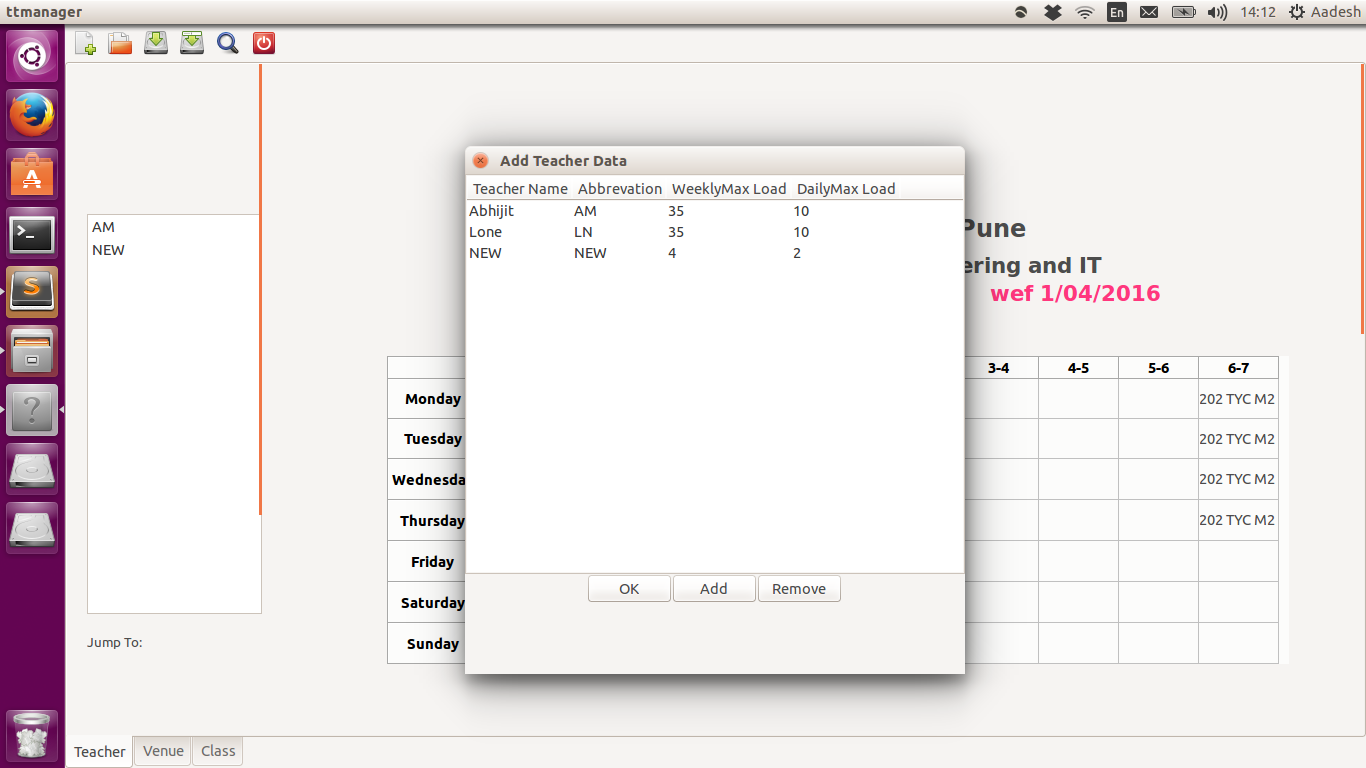
\includegraphics[width=160mm]{5.png}
	\caption{Teacher data entry}
\end{figure}

An example of venue data entry.
\begin{figure}[ht!]
	\centering
	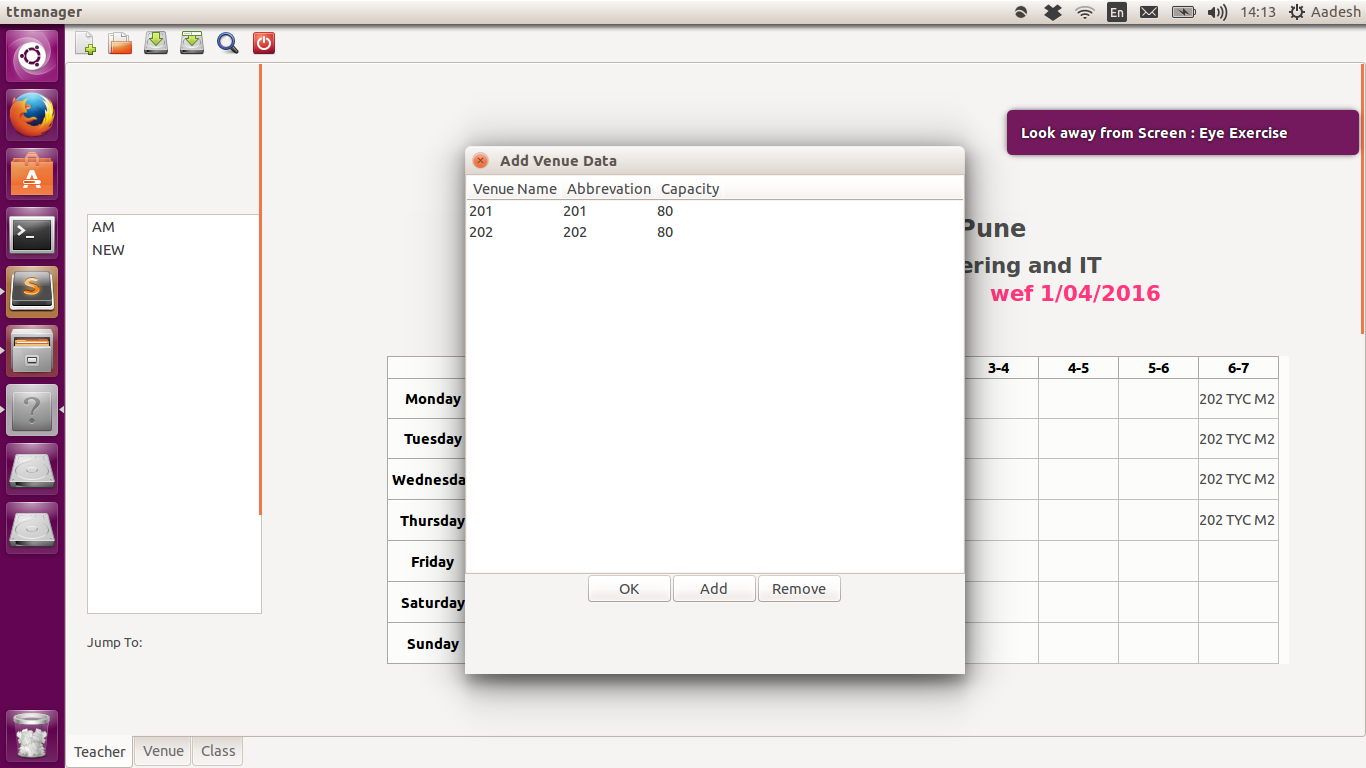
\includegraphics[width=160mm]{6.png}
	\caption{Venue data entry}
\end{figure}

\newpage
An example of class data entry.
\begin{figure}[ht!]
	\centering
	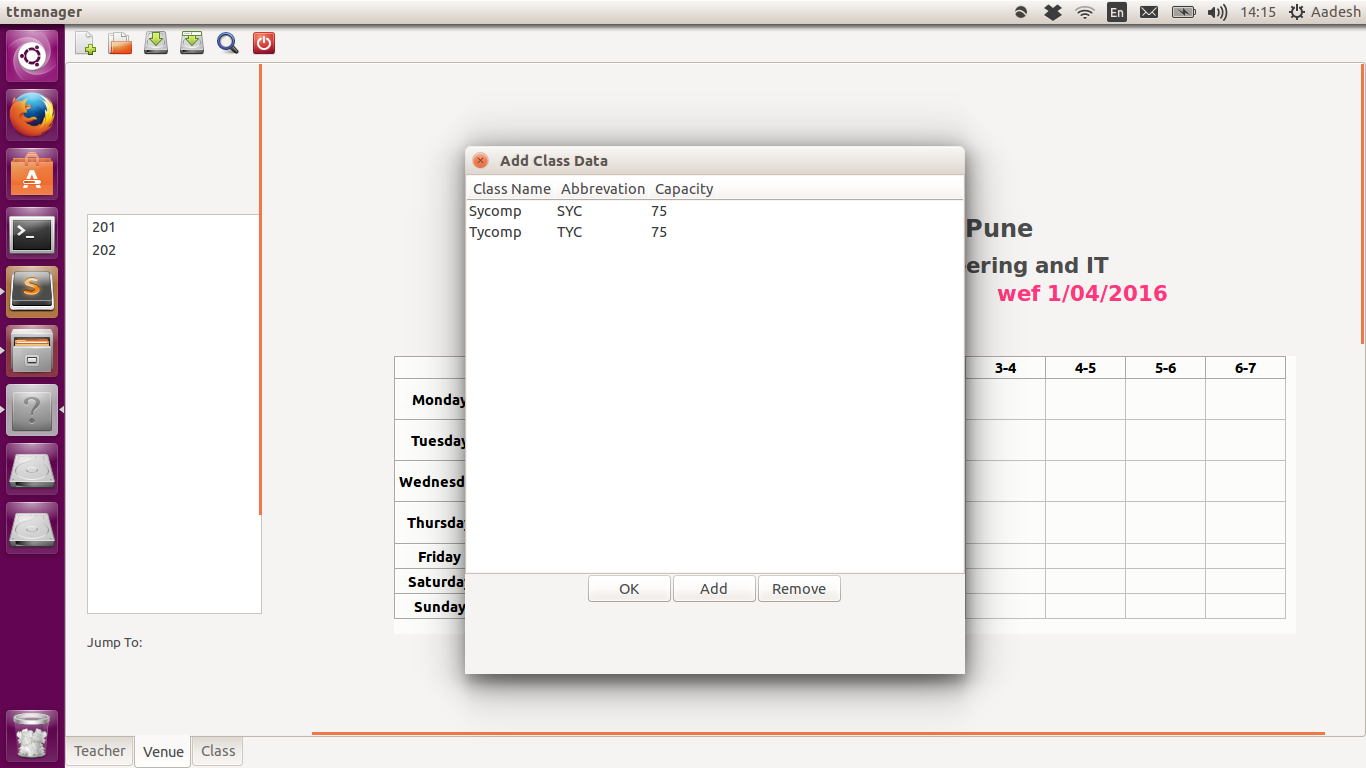
\includegraphics[width=160mm]{7.png}
	\caption{Class data entry}
\end{figure}

An example of subject data entry.
\begin{figure}[ht!]
	\centering
	 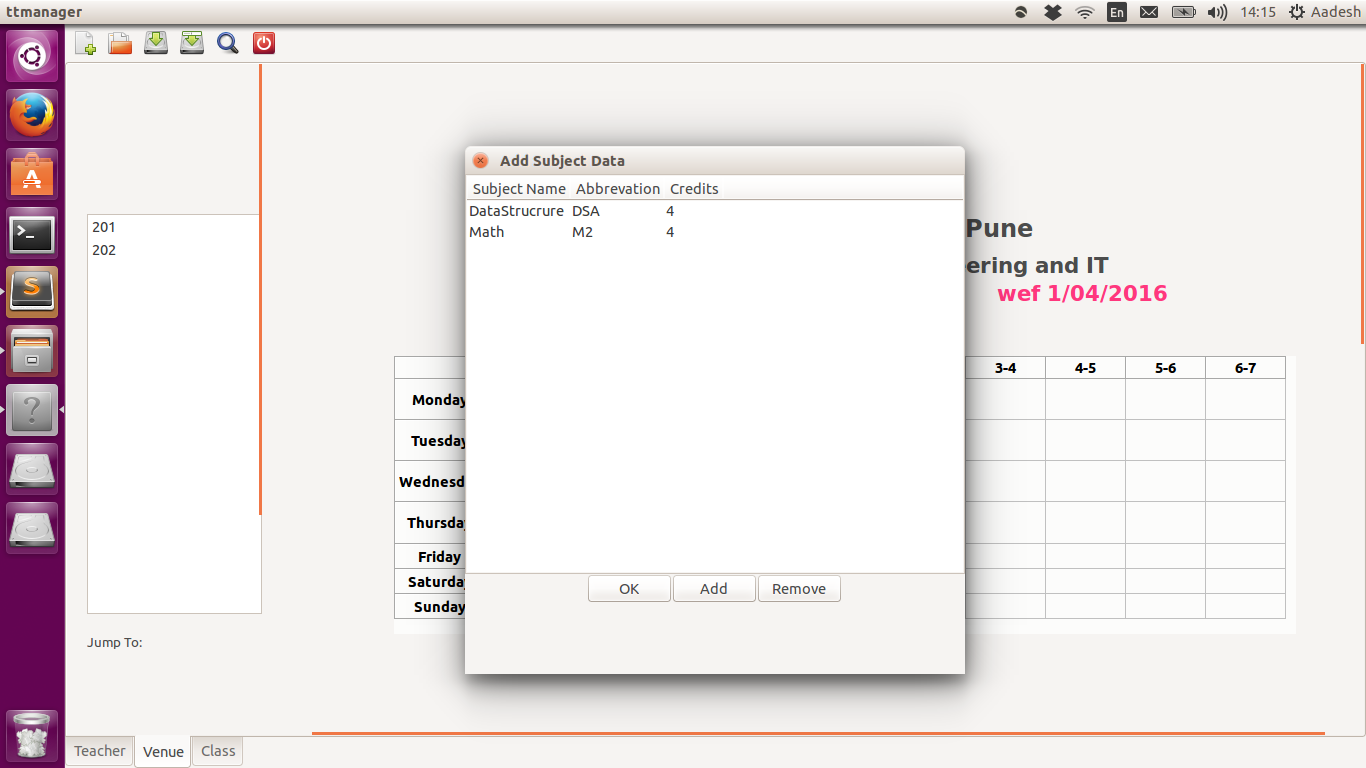
\includegraphics[width=160mm]{8.png}
	\caption{Subject data entry}
\end{figure}

\newpage
User can open/save partial timetable.
\begin{figure}[ht!]
	\centering
	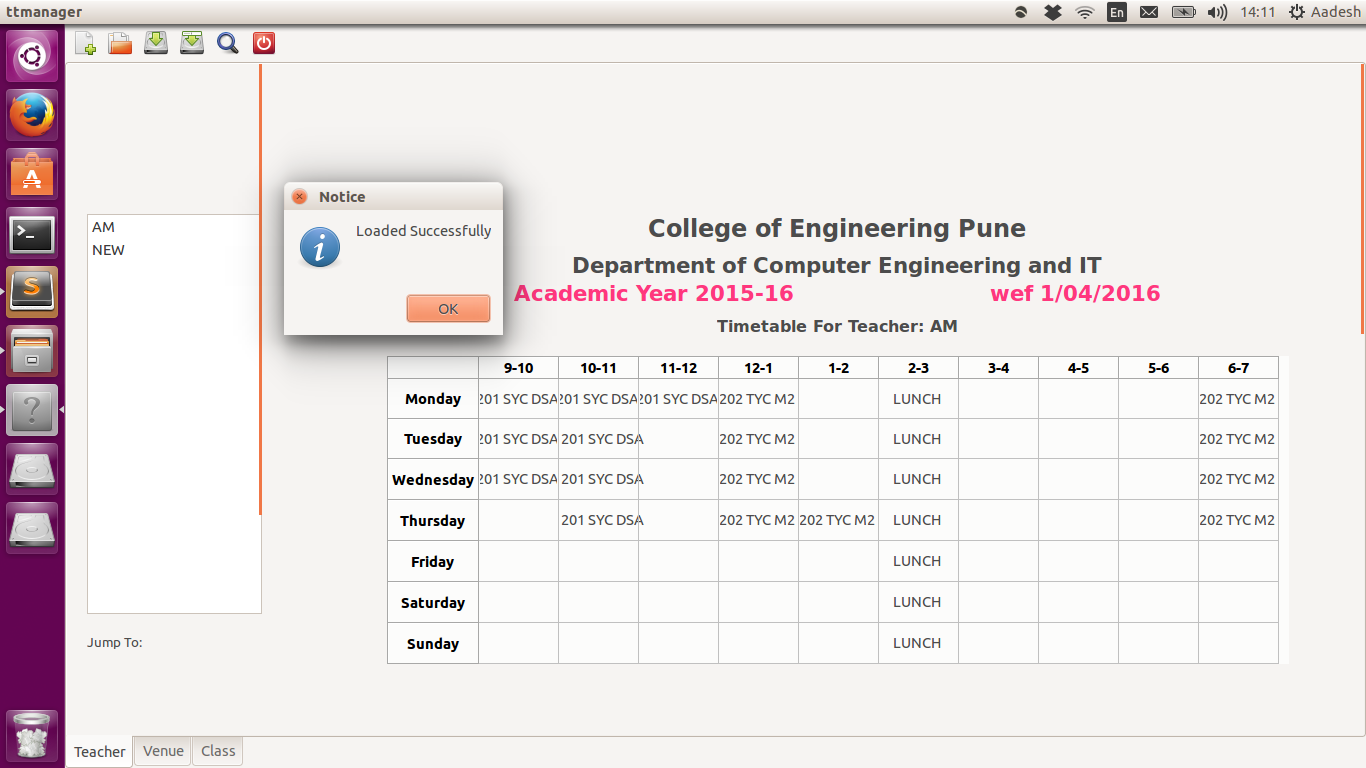
\includegraphics[width=160mm]{4.png}
	\caption{Opening of saved timetable}
\end{figure}

Pop-up boxes are used to take input from the grid. Data gathered from all these UI components is fed to back-end to initialise the timetable. Left-Panel provides easy to navigate mechanism. Double-clicking on an item scrolls to that timetable on current screen. Wxpython provides \textit{wx.lib.scrolledpanel} class for scrollable panels.

\newpage
\section{Back-end}
All data is manipulated by python scripts. \textit{Teacher, Venue, and Classes} are the User-defined class. Every teacher, venue and class involved in the timetable is an instance of these classes. These instances are stored in global lists \textit{all\_teachers}, \textit{all\_venues} and \textit{all\_classes} respectively.
These classes have methods such as can add, \textit{add\_entry}, \textit{remove\_entry} which are slightly different for each class.
% \begin{enumerate}
% \item Check teacher slot, if not available throw error and return control.
% \item If available, check teacher workload less than maximum workload.
% \item If no, show warning, goto 5.
% \item If yes, increment teacher workload, goto 5.
% \item Check venue slot, if not available remove teacher entry, throw error and return control.
% \item If available, check venue capacity less than class size.
% \item If no, show warning, goto 9.
% \item If yes, goto 9.
% \item Check class slot, if not available remove teacher and venue entry, throw error and return control.
% \item If available, entry is added to timetable and return control.
% \end{enumerate}
% {\bfseries Algorithm to insert a normal entry:}

\begin{algorithm}[H]
  \eIf{teacher slot available}{
     \eIf{teacher workload less than maximum workload}{
     		increment teacher workload\;
	   }{
	   		add warning\;
	   }
	   \eIf{venue slot available}{
     		\eIf{venue capacity less than class size}{
     			show warning\;
		   }

			\eIf{class slot available}{
		     		add entry to timetable\;
		     		return\;
			   }{
			   		remove teacher entry\;
			   		remove venue entry\;
			   		throw error and return\;
			   }  	 	
	   }{
	   		remove teacher entry\;
	   		throw error and return\;
	   }
   }{
   throw error and return\;
  }
 \caption{Algorithm to insert a entry:}
\end{algorithm}

% \newpage


{\bfseries Algorithm to add new teacher / venue / class:}

\begin{algorithm}[H]
 % \KwData{teacher/venue/class name to be added}
 % \KwResult{Object corresponding to given name}
 % initialization\;
 % \While{not at end of this document}{
 %  read current\;
  \eIf{object corresponding to name exists}{
   return it\;
   }{
   create instance of Teacher/Venue/Class depending upon type of Data\;
   push the instace into the global list of objects\;
   return the created object\;
  }
 % \caption{Algorithm to add new teacher / venue / class}
\end{algorithm}


% \begin{enumerate}
% \item Get the objects corresponding to the entry.
% \item For teacher and venue, empty that slot. For class check further.
% \item Check if entry is related to whole class or batch.
% \item If related to class, empty that slot.
% \item If related to batch, remove entry corresponding to that batch from the slot.
% \item Decrease the workload count
% \end{enumerate}
{\bfseries Algorithm to remove a entry:}

\begin{algorithm}[H]
 % \KwData{entry to be removed}
Get the objects corresponding to the entry\;
 % \While{not at end of this document}{
 %  read current\;
  \eIf{object type is teacher or venue}{
   empty that slot\;
   }{
     \eIf{entry is related to whole class}{
	   empty that slot\;
	   }{
	   remove entry corresponding to that batch from the slot\;
	   }
  }
Decrease the workload count\;
 % \caption{Algorithm to remove a entry:}
\end{algorithm}


\newpage
{\bfseries Algorithm to find venue utilization:}
% \begin{enumerate}
% \item Get all venue objects from \textit{globaldata.all\_venues}.
% \item For each object, on each working day check all lecture slots.
% \item For each non-empty entry increment the count corresponding to that venue.
% \item Find utilization relative to total available time slots.
% \end{enumerate}

\begin{algorithm}[H]
Get all venue objects from \textit{globaldata.all\_venues}\;
\While{there is next object}{
	get next object\;
	check all lecture slots on each working day\;
	for each non-empty entry increment count corresponding to that venue\;
	find utilization relative to total available time slots\;
}
 % \caption{Algorithm to find venue utilization:}
\end{algorithm}

{\bfseries Algorithm for ods export:}
% \begin{enumerate}
% \item Use the styling\_reference ods file for styling.
% \item Get save file path from user through file select box.
% \item Create three sheets named teacher, venue and class using ezodf and add to the notebook.
% \item Populate the spreadsheet for each teacher, venue and class by traversing the matrix associated with it.
% \item Use styling classes from the reference file.
% \item Save the file in user specified path.
% \end{enumerate}

\begin{algorithm}[H]
\eIf{\textit{styling\_reference.ods} file exists}{
Use the \textit{styling\_reference.ods} file for styling\;
Get save file path from user through file select box.\;
Create three sheets named teacher, venue and class using ezodf and add to the notebook.\;
Populate the spreadsheet for each teacher, venue and class by traversing the matrix associated with it.\;
Use styling classes from the reference file\;
Save the file in user specified path\;
	
}{
	show error and return\;
}
% \caption{Algorithm for ods export:}
\end{algorithm}

\newpage
{\bfseries Algorithm to verify constraints:}
% \begin{enumerate}
% \item Get all class objects from \textit{globaldata.all\_classes}.
% \item For each class check if every batch has lunch break on each working day.
% \item If not add a warning to global warnings list.
% \item For each class check if it satisfies the workload conditions or not.
% \item If not add a warning to global warnings list.
% \item For each class check if no of hours for each subject has been satisfied or not.
% \item If not add a warning to global warnings list.
% \item Get all teacher objects from \textit{globaldata.all\_teachers}.
% \item For each teacher check if every batch has lunch break on each working day.
% \item If not add a warning to global warnings list.
% \end{enumerate}


\begin{algorithm}[H]
\For{each class in \textit{globaldata.all\_classes}}{
  \eIf{every batch as lunch break on each working day}{
   }{
   add warning to global warning list\;
  }
  \eIf{workload of class is within limits}{
   }{
   add warning to global warning list\;
  }
  \eIf{no of hours for each subject satisfied}{
   }{
   add warning to global warning list\;
  }
}
\For{each teacher in \textit{globaldata.all\_teachers}}{
  \eIf{lunch break on each working day}{
   }{
   add warning to global warning list\;
  }
}
 % \caption{Algorithm to remove a entry:}
\end{algorithm}


% \newpage
Teacher and Classes class have additional methods to add / remove lunch. A lunch entry is treated differently than normal lecture entry. The Classes class has another special method valid\_lunch\_break, it is used to verify that all classes and batches have valid lunch breaks. 

\newpage
{\bfseries Algorithm to insert lunch entry:}

% \begin{enumerate}
% \item Check class (or batch) slot or teacher slot.
% \item If available entry is added to the class (or batch) or teacher.
% \item If not available, error is thrown and return control.
% \end{enumerate}

\begin{algorithm}[H]
\eIf{class slot or teacher slot available}{
	add entry to class or teacher\;
}{
	throw error\;
	return\;
}
 % \caption{Algorithm to find venue utilization:}
\end{algorithm}

A wrong entry causes Exception. In that case, its handled and its affects are undo-ed. There are 4 types of Exceptions ExistingEntry Exception, ExtraWorkLoad Exception, LimitForSubject Exception and DailyWorkLoad Exception.
\begin{enumerate}
\item {\bfseries ExistingEntry Exception :}  When the current entry clashes with existing timetable. 
\item {\bfseries ExtraWorkLoad Exception :} When the current entry exceeds the weekly workload of teacher.
\item {\bfseries LimitForSubject Exception :}  When the current entry exceeds the weekly no of lectures for a subject.
\item {\bfseries DailyWorkLoad Exception :}  When the current entry exceeds the daily workload of teacher.
\end{enumerate}

\newpage Hard constraint violation is not permitted where as soft-constraint violation causes warning which is saved in global warnings section. These global warnings are stored in file on filesystem. User can remove warnings from the file (which he/she chose to ignore). The warnings can be refreshed which causes the system to check all constraints and build the warning list again.

\textit{pickle} module is used to save the timetable on filesystem. It allows to save / open the timetable by dumping the in-memory contents on the disk. Exporting the timetable in ods, pdf and html formats is possible. Python modules \textit{ezodf} and \textit{pdfkit} are used to export the timetable. \textit{styling\_reference} is used as a reference style for the ods export.

%\subsection{Vorpal blade}
%And this is a subsection.			


%_____________________________________________________________________________________________ 
 
 
